\documentclass[10pt,landscape]{article}
\usepackage{amssymb,amsmath,amsthm,amsfonts}
\usepackage{multicol,multirow}
\usepackage{calc}
\usepackage{ifthen}
\usepackage{tikz}
\usepackage[landscape]{geometry}
\usepackage[colorlinks=true,citecolor=blue,linkcolor=blue]{hyperref}


\ifthenelse{\lengthtest { \paperwidth = 11in}}
    { \geometry{top=.5in,left=.5in,right=.5in,bottom=.5in} }
	{\ifthenelse{ \lengthtest{ \paperwidth = 297mm}}
		{\geometry{top=1cm,left=1cm,right=1cm,bottom=1cm} }
		{\geometry{top=1cm,left=1cm,right=1cm,bottom=1cm} }
	}
\pagestyle{empty}
\makeatletter
\renewcommand{\section}{\@startsection{section}{1}{0mm}%
                                {-1ex plus -.5ex minus -.2ex}%
                                {0.5ex plus .2ex}%x
                                {\normalfont\large\bfseries}}
\renewcommand{\subsection}{\@startsection{subsection}{2}{0mm}%
                                {-1explus -.5ex minus -.2ex}%
                                {0.5ex plus .2ex}%
                                {\normalfont\normalsize\bfseries}}
\renewcommand{\subsubsection}{\@startsection{subsubsection}{3}{0mm}%
                                {-1ex plus -.5ex minus -.2ex}%
                                {1ex plus .2ex}%
                                {\normalfont\small\bfseries}}
\makeatother
\setcounter{secnumdepth}{0}
\setlength{\parindent}{0pt}
\setlength{\parskip}{0pt plus 0.5ex}
% -----------------------------------------------------------------------

\title{QF1100 Midterms Cheatsheet}

\begin{document}

\raggedright
\footnotesize

\begin{center}
     \Large\textbf{QF1100 Midterms Cheatsheet}     
\end{center}
\begin{multicols}{3}
\setlength{\premulticols}{1pt}
\setlength{\postmulticols}{1pt}
\setlength{\multicolsep}{1pt}
\setlength{\columnsep}{2pt}

\section{Accumulation function and Interest}
\subsection{Accumulation function}
If V(t) is the value of an investment at time t, the ratio
\[a(t)=\frac{V(t)}{V(0)}\] is the accumulation function. a(t) is a measure of how good the investment is. a(1) = 1
\subsection{Cashflow Diagram}
A cash flow diagram visualises a(t). The lower half of a cashflow diagram denotes time, while the upper half denotes payments.

\centering
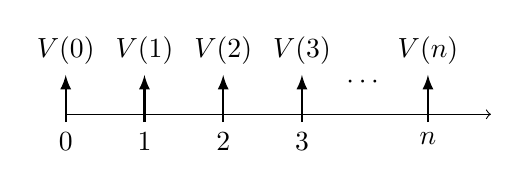
\begin{tikzpicture}
    \draw[->] (0,0) -- (5.4,0);
    \foreach \X in {0,...,3}
    {\draw[thick,-latex] (\X,-0.1) node[below]{$\X$} -- ++(0,0.6) node[above]{$V(\X)$};}
    \draw[thick,-latex] (4.6,-0.1) node[below]{$n$} -- ++(0,0.6) node[above]{$V(n)$};
    \node at (3.8,0.4) {$\cdots$};
\end{tikzpicture}

\raggedright
\subsection{Simple and Compound Interest}
\emph{Simple interest}: \(a(t) = 1 + tr\%, for\; t \geq 0\)\\
\emph{Compound interest}: \(a(t) = (1 + r\%)^t, for\; t \geq 0\)

\subsection{Frequency of Compounding}
A \emph{nominal} interest rate of r\% is compounded p times annually (or convertible p-thly) if the year is divided into p equal periods and interest is paid over each period is $\frac{r\%}{p}$. p is the \emph{frequency of compounding.}\\
If the nominal interest rate of r\% is compounded p times annually, the effective interest rate is
\[r_{e\%}=(1+\frac{r\%}{p})^p - 1\]\\
The accumulation function is
\[a(t) = (1+r_{e\%})^t = (1+\frac{r\%}{p})^{pt}\]\\
2 nominal interest rates are said to be \textbf{equivalent} if and only if they yield the same interest rate, i.e.
\[(1+\frac{r^{(p)}}{p})^p = (1+\frac{r^{(q)}}{q})^q\]\\
$r^{(p)}$ is the nominal interest rate compounded p-thly annually

\subsection{Continuous Compounding}
For a fixed nominal interest rate r, the more we increase the frequency of compounding, the larger the effective interest rate.
When the frequency of compounding tends to infinity, the interest is \emph{compounded continuously}
\[1+r_e = \lim\limits_{p \to \infty}(1+\frac{r}{p})^p=e^r\]\\
Correspondingly, the accumulation function is
\[a(t)=(1+r_e)^t=e^{rt}\]
\subsection{Force of Interest}
The \textbf{force of interest} at time t, of an investment product with activation function a(t), is
\[\delta(t) = \frac{a'(t)}{a(t)}=[ln(a(t))]'\]
Suppose an investment product accumulates like continuously compounded interests, i.e. $a(t)=e^{\delta t}$, then $\delta(t)=\frac{\delta e^{\delta t}}{e^{\delta t}}=\delta$.\\
\textbf{One is indifferent between an investment product with $\boldsymbol{\delta(t)}$ as force of interest at time \emph{t}, and a deposit with nominal interest rate of $\boldsymbol{\delta(t)}$ compounded continuously}
From definition of force of interest, 
\[a(t) = \exp{\int_0^t\delta(\mathrm{u})\mathrm{du}}\]\\
If $0<s<t$, then\\
\[a(s, t)=\frac{a(t)}{a(s)}=exp{\int_s^t\delta(\mathrm{u})\mathrm{du}}\]\\
is the value of investment at time \emph{s} when \$1 is invested at time \emph{s}. Hence, the \emph{principle of consistency}: \\For $0<t_0<t_1<t_2<...<t_n$,
\[a(t_0,t_n)=a(t_0,t_1)a(t_1,t_2)...a(t_{n-1},t_n)\]
\section{Present Value and Equivalence}
\subsection{Present Value and Time Value}
Let a(t) be the accumulation function of a bank deposit. Let c be an amount guaranteed to receive T time periods later. Then, the \emph{present value} of c is
\[\frac{c}{a(T)}\]
For a cash flow consisting of a series of payments, with $c_i$ received at time $t_i$,
\[\Vec{C}={(c_1, t_1), (c_2, t_2),..., (c_n, t_n)}\]

the \emph{present value},$PV(\Vec{C})$, is defined by
\[PV(\Vec{C})=\displaystyle\sum_{i=1}^n\frac{c_i}{a(t_i)}\]
Time value of $\Vec{C}$ at time t, $TV_t(\Vec{C})$ is given by
\[TV_t(\Vec{C}) = PV(\Vec{C})\times a(t)\]
Suppose effective annual interest rates are constant at \emph{r}, and \emph{t} is measured in years, then $a(t) = (1 + r)^t$. Then,
\[PV(\Vec{C}) = \displaystyle\sum_{i=1}^n\frac{c_i}{(1+r)^{t_i}}\;and\;TV_t(\Vec{C}) = \displaystyle\sum_{i=1}^n\frac{c_i}{(1+r)^{t_i-t}}\]
If $t_i = i - 1$, then 
\[\Vec{C} = {(c_1, t_1), (c_2, t_2),..., (c_n, t_n)} = {(c_1, 0), (c_2, 1),..., (c_n, n-1)}\]
\[= (c_1, c_2,...,cn)\]
\subsection{Principle of Equivalence}
Two cash flows are \textbf{equivalent} if and only if they have the same present value.
\subsection{Internal Rate of Return(IRR)}
Given a cash flow $\Vec{C}={(c_1, t_1), (c_2, t_2),..., (c_n, t_n)}$, the equation
\[PV(\Vec{C})=\displaystyle\sum_{i=1}^n\frac{c_i}{(1+r)^{t_i}} = 0\]
is known as the \textbf{equation of value}.\\
Any non negative solution, r, for the equation of value is known as the yield, or IRR. 
IRR is the prevailing interest rate such that one is indifferent between $\Vec{C}$ and \$0
\section{Annuities}
An \textbf{annuity} is a series of payments made at regular intervals. \\
A \textbf{perpetuity} is an annuity with infinite payments.
\section{Loans}
Loans are repaid by a series of installment payments made at periodic intervals. If \emph{L} is the amount of loan taken at time \emph{t} = 0 and $\Vec{C}={(c_1, t_1), (c_2, t_2),..., (c_n, t_n)}$ is the series of repayments, then
\[L=PV(\Vec{C})\]
\subsection{Loan Balance}
Loan Balance immediately after the \emph{m}-th installment is paid is the Time Value at \emph{t=m} of the remaining \emph{(n-m)} installment payments.

Sometimes, we need to determine n based on the Loan itself. 
\[\Vec{C} = \overbrace{(A, A, ..., \underbrace{A+B}_\text{\emph{n}-th payment})}^\text{\emph{n} payments} \]
To find n, find the largest n such that \emph{PV($\Vec{C}$)} of \emph{n} payments of \emph{A} $\leq$ \emph{L} and \emph{PV($\Vec{C}$)} of \emph{n} + 1 payments of \emph{A} $>$ \emph{L}

\section{Bonds}
Bonds are issued by governments/corporations that want to borrow money. It is a written contract between issuer (borrower) and investors (lenders/bond holders), and can be freely traded before the maturity date.
\subsection{Bond Risks}
Interest Rate Risk: Risk due to prevailing fluctuating interest rates (may be more profitable to put money in bank deposit vs buy the bond)\\
Default Risk: Credit-worthiness of bond issuer Risk that the bond issuer will default on coupon payments\\
Liquidity Risk: Risk due to liquidity/ease of buying and selling bond
\textbf{We assume these risk do not exist i.e. interest rates are constant, no default/liquidity risk}
\subsection{Basic Bond Terminology}
\begin{enumerate}
    \item \textbf{F}: Face value/par value of bond - amount based on which periodic interest payments are computed
    \item \textbf{R}: Redemption value/maturity value of bond - amount to be repaid at the end of the loan. Typically same as F
    \item \textbf{c\%}: Coupon rate - bond's interest payments, represented as percentage of par value, to be paid regularly to investors during the term of the loan
    \item \textbf{Maturity Date}: Or redemption date - date on which the loan will be fully repaid. Additionally, \textbf{m} denotes the no. of coupon payments per year, and \textbf{n} denotes the total no. of coupon payments
\end{enumerate}
\textbf{Important: When the bond is issued, the information is specified and FIXED throughout the duration of the loan}\\
Cash flow of the bond is given by
\[\Vec{C}=\left((-P, 0), (\frac{c\%F}{m}, \frac{1}{m}),(\frac{c\%F}{m}, \frac{2}{m}),\dotsc, (\frac{c\%F}{m}+R, \frac{n}{m})\right)\]
\textbf{Subsequently, we assume $R=F$}
\subsection{Bond yields}
For any time \emph{t} in the lifetime of the bond, the nominal yield of the bond is the nominal internal rate of return compounded \emph{m} times per annum of holding the bond from time \emph{t} to maturity.\\
If $P(t)$ is the price of bond at time \emph{t}, then nominal yield, $\lambda(t)\%$, satisfies
\[P(t)=\overbrace{\frac{R}{\left(1+\frac{\lambda(t)\%}{m}\right)^{n-tm}}}^\text{Redemption value \emph{R} discounted}+\overbrace{ \displaystyle\sum_{i=1}^{n-tm}\frac{c\%F/m}{\left(1+\frac{\lambda(t)\%}{m}\right)^i}}^\text{final \emph{n-tm} coupon payments}\]
If $R=F$, then
\[P(t)=F\left[\frac{1}{\left(1+\frac{\lambda(t)\%}{m}\right)^{n-tm}}+\frac{c}{\lambda(t)}\left(1-\frac{1}{\left(1+\frac{\lambda(t)\%}{m}\right)^{n-tm}}\right)\right]\]
\[=F+F\left(\frac{c-\lambda(t)}{\lambda(t)}\right)\left[1-\frac{1}{\left(1+\frac{\lambda(t)\%}{m}\right)^{n-tm}}\right]\]

Bond is priced at time \emph{t}
\begin{enumerate}
    \item at a \emph{premium} if $P(t)>F$ and iff $c>\lambda(t)$
    \item at \emph{par} if $P(t)=F$ and iff $c=\lambda(t)$
    \item at a \emph{discount} if $P(t)<F$ and iff $c<\lambda(t)$
\end{enumerate}
Effective yield,$\lambda_e(t)\%$, satisfies
\[P(t)=\frac{R}{(1+\lambda_e(t)\%)^{\frac{n}{m}-t}}+\sum_{i=1}^{n-tm}\frac{c\%F/m}{(1+\lambda_e(t)\%)^{\frac{i}{m}}}\]
Note: $P(\frac{n}{m})=R$
\subsection{Price-yield Relationship}
Price $P(t)$ of the bond at time \emph{t} is a decreasing function of the nominal yield $\lambda(t)$. Furthermore, this graph is convex.\\
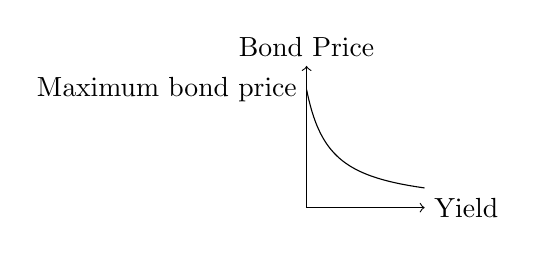
\begin{tikzpicture}[scale=0.3]
    \draw[->] (0,0) -- (5,0) node[right] {Yield};
    \draw[->] (0,0) -- (0,6) node[above] {Bond Price};

    \draw plot [samples=100, domain=0:5] (\x,{5/(\x+1)});
    
    % Label y-intercept
    \node[anchor=east] at (0,5) {Maximum bond price};
\end{tikzpicture}
\subsection{Common types of bonds}
\emph{Zero coupon bond}: a bond that pays no coupons. At any time \emph{t}, the price $P(t)$ and effective yield $\lambda_e(t)\%$ of a $N$-year zero-coupon bond with maturity value $R$ satisfies
\[P(t)=\overbrace{\frac{R}{(1+\lambda_e(t)\%^{N-t}}}^\text{Discount $R$ by $N-t$ years}\]
\emph{Perpetual bond} or \emph{consol}: a bond that never matures. At any time $t > 0$, the price $P(t)$ and nominal yield $\lambda(t)$\% of a perpetual bond with coupon $c$ paid $m$ times annually satisfies
\[P(t)=\frac{cF}{\lambda(t)}\]
\subsection{Pricing a bond}
To price a bond, we make the following simplifying assumptions
\begin{itemize}
    \item Interest rates constant over lifetime of bond $\iff$ yield is constant (reasonable if economic conditions are stable)
    \item Yield at any point of time = interest rates (reasonable if no significant default/liquidity risks). Then, price of bond = PV
\end{itemize}
\textbf{Given this, we can price the bond at every point of time by replacing $\lambda(t)$ by current interest rates}
\section{Sensitivity of bond prices to interest rates}
\subsection{Macaulay Duration and Average Holding Times}
\emph{Macaulay duration} of any cash flow $\Vec{C} = ((c_1,t_1), (c_2,t_2),\dotsc,(c_n,t_n))$ is the quantity
\[D=\frac{\displaystyle\sum_{i=1}^nt_i\cdot PV(C_i)}{PV(\Vec{C}})=\sum_{i=1}^nw_it_i\]
where $PV(C_i)$ is the present value of $C_i$ and $w_i=\frac{PV(C_i)}{PV(\Vec{C})}$. The Macaulay duration is the average time each dollar in $PV(\Vec{C}$ needs to be held before it can be redeemed by investor.\\
For infinite cash flow $\Vec{C} = ((c_1, t_1), (c_2, t_2),\dots)$:
\[D=\frac{\displaystyle\sum_{i=1}^\infty t_i\cdot PV(C_i)}{PV(\Vec{C})}\]
For zero-coupon bond:\\
\[D=t_n\]
For bond \emph{redeemable at par}($R=F$) and pays $n$ coupons at a frequency of $m$ payments a year. Suppose constant nominal bond yield $\lambda\%$ and coupon rate $c\%$. Cash flow is given by
\[\Vec{C}=\left(\left(\frac{c\%F}{m}, t_1\right),\dotsc,\left(\frac{c\%F}{m}, t_{n-1}\right),\left(\frac{c\%F}{m}+F, t_n\right)\right)\]
where $t_i=\frac{i}{m}$, such that
\[D=\frac{1}{P}\left[\displaystyle\sum_{i=1}^n\overbrace{\frac{\frac{c\%F}{m}}{\left(1+\frac{\lambda\%}{m}\right)^i}}^{PV(C_i)}\cdot\overbrace{\frac{i}{m}}^{t_i}+\overbrace{\frac{F}{\left(1+\frac{\lambda\%}{m}\right)^n}\cdot\frac{n}{m}}^{PV(R)\times t_n}\right]\]
where
\[P=\sum_{i=1}^n\frac{\frac{c\%F}{m}}{\left(1+\frac{\lambda\%}{m}\right)^i}+\frac{F}{\left(1+\frac{\lambda\%}{m}\right)^n}\]
Then,
\[D=\frac{1+\frac{\lambda\%}{m}}{\lambda\%}-\frac{1+\frac{\lambda\%}{m}+n\left(\frac{c\%}{m}-\frac{\lambda\%}{m}\right)}{c\%\left[\left(1+\frac{\lambda\%}{m}\right)^n-1\right]+\lambda\%}\]
For a perpetual bond ($n\rightarrow\infty$),
\[D=\frac{1+\frac{\lambda\%}{m}}{\lambda\%}\]
If bond priced at par ($\lambda=c$),
\[D=\frac{1+\frac{c\%}{m}}{c\%}\left(1-\frac{1}{\left(1+\frac{c\%}{m}\right)^n}\right)\]
\subsection{Modified Duration and Sensitivity}
Modified duration measures the sensitivity per unit dollar of the present value $P$ of a cash flow to interest rates $\lambda$
\[D_M=\frac{\left(\frac{\mathrm{d} P}{\mathrm{d}\lambda}\right)}{P}\]
By differentiating $P$ wrt $\lambda$,
\[\frac{\mathrm{d}P}{\mathrm{d}\lambda}=\frac{1}{1+\frac{\lambda}{m}}DP\]
Then,
\[D_M=\frac{1}{1+\frac{\lambda}{m}}D\]
By linear approximation,
\[P(\lambda+\Delta\lambda)\approx P(\lambda)-(D_MP)\cdot\Delta\lambda\]
The corresponding change in P,$\Delta P$ is
\[\Delta P\approx-(D_MP)\cdot \Delta\lambda\]
\end{multicols}

\end{document}
